% -----------------------------------------------
% Vlastní text práce (kapitoly práce)
% -----------------------------------------------

% -----------------------------------------------
\chapter{Calibration of astroparticle detectors}
% -----------------------------------------------
Calibration is a process, which we perform to obtain relationships between measured values by a tested device and values given by ethalon. These relationships may be specified by calibration constants, functions or by other mathematical relations. The tested devices can be also calibrated relatively to each other.
\par
%In case of astroparicle detection, we mostly need to ,  , 
\section{Absolute calibration}
% -----------------------------------------------
The term absolute calibration can be specified as a measurement process, which results in obtaining reference between the detector's responsivity and the defined value of some physical quantity induced by an external source. In case of detectors consisting of PMTs or PMT based cameras it is reference between optical power seen by detector and its output photocurrent. Due to the PMT's linearity principle we can define this reference by one constant for every PMT or pixel. However, in real applications, other corrections must be made.

\par
Good example of absolute calibration light sources are large-aperture light drums, which were used at Pierre Auger for fluorescence telescopes calibration. The drum's inner surface is coated with a diffuser and a UV LED is used as a light source with defined power. This concept provides a homogeneous intensity for absolute calibration of large mirrors along with the PMT camera. 

\par
In many cases the absolute calibration is a complicated process, and thus it is done less frequently than the relative calibration.

% -----------------------------------------------
\section{Relative calibration}
The term relative calibration refers to comparing the response on the same signal between two detectors or to propagating the constants from absolute calibration over time.
In this thesis we mainly use this term to describe the comparing the signal response between PMTs, which belong to the same FAST telescope. 
\par
The relative calibration has a lesser requirement on instruments and methods than the absolute calibration. For example we don't have to illuminate the PMTs with well defined intensity, the only requirement is to illuminate each of them with the same amount. 


%--------------------------------------------
\section{FAST calibration}
%-----------------------------------------------------
FAST telescope calibration techniques are yet under development. It is necessary to calibrate PMTs both in absolute and relative way, but also the entire telescope as optoelectronic system with mirrors and PMTs. However, the mirrors also suffer from various effects, and thus their reflectance needs to be tested sometimes.
% ----------------------------------------------------
\subsection{Flasher}
As was mentioned before, the FAST telescope is equipped with UV LED flasher, which is used to generate light pulses. Relative calibration of PMTs by flasher is performed during every shift.
\subsection{YAP pulser}
YAP pulser consists of radioactive isotope of $\textrm{Am-241}$ and YAP scintillator crystal. Due to the long half life of $\textrm{Am-241}$, the YAP pulser could be used as stable low-intensity UV source. 
It is mainly used for absolute calibration of PMTs. During the calibration the YAP pulser is mounted directly on the window of the PMT.

\subsection{Homogeneous light source}
Another way of calibration is to use a stable light source mounted into the IS. However, this homogeneous light source is not able to produce homogeneous illumination for the entire FAST's aperture.  
\par
To perform a relative calibration with the mirrors and the entire optical system included, it would be necessary to XY scan the aperture with the homogeneous light source, but this would be very difficult to implement.   

\par
The other and more practical way is to illuminate the telescope's aperture from few different positions and obtain relative responsivity ration constants for every PMT (not final calibration constants). By comparing these measured responsivity ration constants with its theoretical counterparts produced by simulations of illuminating the FAST's optical system, we are able to calculate the relative calibration constants for every PMT.       
\par
The analysis of calibration data acquired by this method are presented in chapter \ref{chap7}.

\par
As a light source for this application is used thermal stabilized UV LED source. The functionality and testing of this source is more discussed in chapter \ref{chap4}.


\begin{figure}[H]
 \centering
 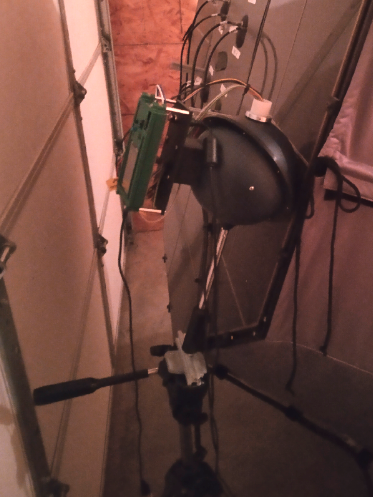
\includegraphics[scale=0.35, angle = 0]{./pictures/CalibMech.png}
 \caption{UV LED source mounted onto the telescope aperture.}
 \label{bottomCal}
 
\end{figure}

\subsection{Drone with light source}
There is a possibility to use a drone to carry the calibration light source. Performing this type of calibration will allow us to scan the FAST's FoV homogeneity from the air. However, this type of calibration is yet under fresh development and has never been performed on the FAST yet.


\begin{figure}[H]
 \centering
 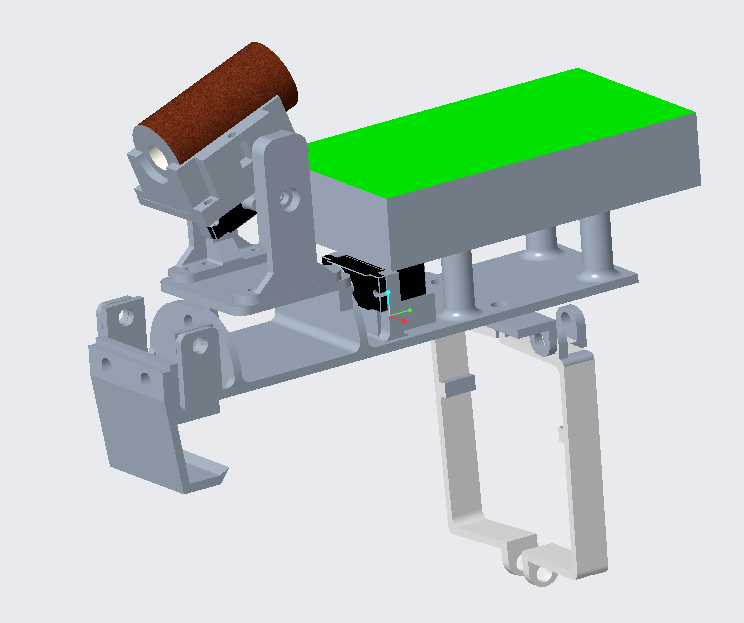
\includegraphics[scale=0.35, angle = 0]{./pictures/teoreticalDesign.png}
 \caption{Initial design of the on-drone calibration apparatus.}
 \label{Drone}
 
\end{figure}


%------------------------------------------------


% -----------------------------------------------



% -----------------------------------------------
% %%%%%%%%%%%%%%%%%%%%%%%% End of file %%%%%%%%%%%%%%%%%%%%%%%%
